% Attack-resilient firmware for single-chip Wi-Fi intrusion alarms.
%
% This compiles with a stock LaTeX install (two-column article). To submit to an IEEE venue,
% replace the preamble down to \begin{document} with \documentclass[conference]{IEEEtran}
% and the \author block with the IEEE form; the body, figures and bibliography port unchanged.
\documentclass[10pt,twocolumn]{article}
\usepackage[a4paper,margin=0.75in,columnsep=0.25in]{geometry}
\usepackage{times}
\usepackage{graphicx}
\usepackage{booktabs}
\usepackage{amsmath}
\usepackage{url}
\usepackage[hidelinks]{hyperref}
\usepackage{abstract}
\usepackage{titlesec}
\titleformat{\section}{\normalfont\large\bfseries}{\thesection}{0.6em}{}
\titleformat{\subsection}{\normalfont\normalsize\bfseries}{\thesubsection}{0.5em}{}
\setlength{\parindent}{1em}
\setlength{\parskip}{0pt}
\pagestyle{plain}

\title{\vspace{-2em}\bfseries Does Core Pinning Isolate the Safety Function on a
Single-Chip Wi-Fi SoC? An Attack-Resilient Intrusion Alarm, Measured and Verified}

\author{MD Humayun\\
\small Department of Computer Science and Engineering\\
\small Sardar Vallabhbhai National Institute of Technology, Surat, India\\
\small \texttt{github.com/mdhumayun7/Smart-Home-Automation}}
\date{}

\begin{document}
\maketitle

\begin{abstract}
\noindent
Consumer intrusion alarms are built almost entirely on single-chip Wi-Fi systems-on-chip, in
which the radio stack, the network stack and the application share one die and one scheduler.
The real-time-security literature shows that on Linux-class industrial devices, pinning the
control task to a separate core keeps its timing stable under wired network floods; whether
that result transfers to a single-chip Wi-Fi SoC, where the attacked radio driver runs on the
same silicon, is untested. We study an ESP32 intrusion alarm whose safety loop (sensing, state
machine, siren) is pinned to the application core and whose network task runs on the other
core behind bounded, non-blocking queues. We contribute: (i) a dual-core firmware with
authenticated commands (HMAC-SHA256 over an NVS-persisted monotonic counter), passive
deauthentication-flood detection and an out-of-band signed fallback alert; (ii) two
machine-checked TLA+ models proving that no network behaviour can disarm the system or block
a safety step, over their full state spaces; (iii) a reproducible, seeded adversarial campaign
of 6{,}000 trials in which command injection up to 20{,}000~msg/s never disarms the device and,
with authentication enabled, never prevents a legitimate command either, while the baseline is
armed by an attacker in every flooded trial; and (iv) a fuzzing campaign of the command parser
under AddressSanitizer that finds no memory-safety or authentication defect. The remaining
claim---that the physical sensor-to-siren latency is invariant to on-chip radio stress---can
only be established on hardware; we specify the measurement apparatus and leave the RF campaign
as the one open step. The firmware, specs, experiments and this paper are a public artifact.
\end{abstract}

\section{Introduction}
A networked intrusion alarm has an unusual priority order. Confidentiality matters, but the
property that defines the device is \emph{availability of the safety function}: when a sensor
fires, the siren must sound within a bounded time, and it must do so \emph{even while the device
itself is under attack}, because an intruder has every incentive to attack it.

Almost all such consumer devices are built on single-chip Wi-Fi SoCs of the ESP32 class, where
the Wi-Fi driver, the TCP/IP stack, the MQTT client and the application all execute on the same
chip under one RTOS scheduler. This differs structurally from the industrial devices studied in
the real-time-security literature, where the control task can be placed on a physically separate
core or co-processor. Fischer \emph{et al.}~\cite{fischer2020} show that on a Linux-class board,
pinning the control task to a dedicated core holds its 1\,ms cycle jitter essentially constant
under wired SYN and ARP floods, and that only a separate co-processor is acceptable for hard
real-time. The natural question for the devices people actually deploy is whether the same
advice---pin the safety task to a core---delivers the same isolation when the \emph{attacked
resource is the on-chip radio driver}, which shares the die and the interrupt controller with
the safety task.

We take an ESP32 intrusion alarm as the object of study. Its safety loop is pinned to the
application core; Wi-Fi, time sync and MQTT run in a task on the other core and communicate with
the safety loop only through two bounded FreeRTOS queues and a mutex-guarded status snapshot
that the safety loop never waits on. On top of this structure we add the security mechanisms a
deployable alarm needs and then ask, with formal methods, simulation and a specified hardware
protocol, whether the isolation actually holds.

\paragraph{Contributions.}
\begin{enumerate}\itemsep0.1em
\item An open dual-core alarm firmware with authenticated commands (HMAC-SHA256 over a
monotonic, reboot-persistent counter), passive deauth/disassoc flood detection, a signed
out-of-band fallback alert over ESP-NOW, and optional PIR+mmWave sensor fusion
(Section~\ref{sec:design}).
\item Two TLA+ specifications, checked exhaustively by TLC: one of the alarm state machine and
command path, one of the safety/network isolation, each mutation-tested to show the properties
are not vacuous (Section~\ref{sec:formal}).
\item A seeded, reproducible adversarial campaign (6{,}000 trials) and a sanitizer-backed fuzzing
campaign of the command parser, with a non-parametric test of latency invariance
(Section~\ref{sec:sim}).
\item A measurement protocol and instrumentation for the one claim that requires silicon---the
physical latency invariance under on-chip radio stress---stated honestly as the open step
(Section~\ref{sec:hw}).
\end{enumerate}

\section{Related Work}
\textbf{Timing isolation under attack and interference.} This is the closest body of work, and its
consistent finding is that spatial separation plus a resource regulator preserves real-time
behaviour. Its consistent platform, however, is large. Fischer \emph{et al.}~\cite{fischer2020}
measure control-task jitter on Linux-class industrial devices under \emph{wired} floods and find
core pinning effective, with a separate co-processor best; the attacked interface there is a
physically separate NIC. Meszl\'enyi \emph{et al.}~\cite{timingiso2025} hold DDS latency and jitter
predictable under heavy interference using priority-based middleware scheduling, AF\_XDP kernel
bypass and dedicated NIC hardware queues on x86 with a PREEMPT-RT kernel. Hoornaert
\emph{et al.}~\cite{mcti2024} co-design CPU-time and memory-bandwidth isolation on a Cortex-A53
MPSoC, switching the interconnect from fair to fixed-priority arbitration on overload, using a
hypervisor and an FPGA-hosted memory scheduler. The mixed-criticality literature these sit in is
surveyed by Burns and Davis~\cite{mcreview2026}, which treats criticality as a scheduling problem
under benign timing assumptions. None of the mechanisms these works rely on---an MMU, a
hypervisor, performance-counter regulation, separate NIC queues---exist on a 240\,MHz
single-chip Wi-Fi SoC. What remains available there is core pinning and queue discipline alone,
and whether that residual mechanism suffices is an open empirical question about a particular
silicon and radio driver.

\textbf{Radio-layer attacks on this device class.} The attack side is established and specifically
demonstrated on this chip family. Carbajal and Jodeiri Akbarfam~\cite{carbajal2026} quantify
deauthentication resilience across open, WPA2, PMF and WPA3 configurations, finding PMF effective
under the conditions tested; the dependent variable is whether the \emph{link} drops. Kremser and
Graffi~\cite{deauther2026} build deauthentication firmware for the ESP32-S3 itself---patching the
compiled image because the ESP-IDF transmit path rejects such frames---showing the attack is cheap
and portable against exactly this hardware. Cayre \emph{et al.}~\cite{espwn2023} reverse-engineer
the ESP32 family's wireless ROM components and inject, alter and jam link-layer traffic from
software, supporting our assumption that radio-layer stress is a realistic in-scope condition.
Crucially, all of this measures the link or the attacker's reach, not whether the victim's
\emph{application} still meets its deadline.

\textbf{ESP32 application-stack security.} Work on this platform measures the latency cost of
MQTT-over-TLS on an ESP32-C3~\cite{mqtttls2026} and runs on-device ML intrusion detection on an
ESP32~\cite{ondevice2026}. Both are valuable, and both optimise transport cost or detection
accuracy rather than treating a safety deadline as the dependent variable; an on-device detector is
itself additional load on the contended chip.

\textbf{Formal verification and fuzzing.} Krichen's survey of formal verification for
IoT~\cite{krichen2023} covers model checking, abstract interpretation and deductive verification
with Event-B, Maude and Simulink tooling, and does not record TLA+~\cite{lamport2002} use for this
device class---still less a TLA+ model of a task-isolation argument. On the fuzzing
side~\cite{fuzzsurvey2022}, the frontier is whole-firmware: Bley \emph{et al.}~\cite{pemu2025}
wrap fuzz inputs in protocol-valid packets to reach deep network-stack code, and
SysFuSS~\cite{sysfuss2026} adds selective symbolic execution when coverage stalls. Our fuzzing is
deliberately narrower---the application-layer command parser in a host harness---and is evidence
for one property with a precise oracle, not a contribution to fuzzing technique.

\begin{table}[t]
\centering\small
\caption{Positioning. No prior work measures a safety deadline on a single-chip Wi-Fi SoC whose own
radio driver is the attacked resource.}
\label{tab:position}
\begin{tabular}{@{}llcc@{}}
\toprule
Work & Platform & \shortstack{Attacked\\resource\\on-die} & \shortstack{Safety\\deadline\\measured} \\
\midrule
Fischer~\cite{fischer2020}      & Linux ind.\ board & no  & yes \\
Meszl\'enyi~\cite{timingiso2025}& x86 PREEMPT-RT    & no  & yes \\
Hoornaert~\cite{mcti2024}       & A53 + hypervisor  & n/a & yes \\
Carbajal~\cite{carbajal2026}    & Wi-Fi testbed     & n/a & no  \\
Kremser~\cite{deauther2026}     & ESP32-S3          & n/a & no  \\
Cayre~\cite{espwn2023}          & ESP32 family      & yes & no  \\
Azhar~\cite{mqtttls2026}        & ESP32-C3          & no  & no  \\
Ieropoulos~\cite{ondevice2026}  & ESP32             & no  & no  \\
\midrule
\textbf{This work}              & \textbf{ESP32}    & \textbf{yes} & \textbf{yes}$^\dagger$ \\
\bottomrule
\end{tabular}

\vspace{0.3em}
{\footnotesize $^\dagger$Logical invariance established here; physical latency invariance is the
specified open step (Section~\ref{sec:hw}).}
\end{table}

\section{System Design}\label{sec:design}
\textbf{Dual-core structure.} The Arduino \texttt{loop} runs the safety function on the
application core: input conditioning (debouncing, a PIR warm-up and 150\,ms confirmation
filter), a five-state arm/disarm machine (exit and entry delays, an alarm timeout), and the
outputs (siren, LEDs, display). A separate task, pinned to the other core, runs Wi-Fi with
retry, NTP, the MQTT client, and event delivery. The two communicate only through a 16-deep
event queue (safety$\rightarrow$network) and a 4-deep command queue (network$\rightarrow$safety),
plus a status snapshot the safety loop copies under a zero-timeout mutex---so the safety loop
never blocks on the network side. The enqueue of an event never blocks either: on a full queue
the oldest is dropped and counted, never silently lost.

\textbf{Authenticated commands.} A command on the MQTT topic is trusted only if it carries a
valid HMAC-SHA256 tag over the string \texttt{VERB:counter}, where the counter must strictly
exceed the highest previously accepted value. The counter is persisted in NVS, so replay
protection survives a reboot. This defeats both forgery (no key, no tag) and replay (no fresh
counter), and lets a signed command safely perform remote disarm, which is otherwise refused.

\textbf{Attack detection and fallback.} A passive promiscuous-mode monitor counts
deauthentication/disassociation frames and raises a \texttt{wifi\_deauth} event when a burst
exceeds a threshold; loss of the link while armed is itself raised as \texttt{link\_lost}. When
MQTT is unreachable, critical events are additionally sent as HMAC-signed, counter-protected
ESP-NOW messages to a second node, which is peer-to-peer and so survives an attack aimed at the
access point. These mechanisms add roughly 3\,KB of flash and 170\,B of RAM over the
unhardened build.

\section{Formal Verification}\label{sec:formal}
We model two properties in TLA+ and check them exhaustively with TLC.

\textbf{State machine and command path.} The first spec models the five states and the command
rules. TLC verifies, over all 25 reachable states, that (i) no unauthenticated remote command
ever disarms the system, (ii) the replay counter never decreases, (iii) the siren is never
active while disarmed, and (iv) the entry delay and the alarm always resolve (no stuck state).

\textbf{Isolation.} The second spec models the two tasks with the network task made maximally
adversarial: it may stall for an unbounded time, be flooded, fail to publish, and crash and
restart, and it is given \emph{no} fairness. The safety task is a loop. TLC verifies, over all
660 reachable states, that in every state the safety step is enabled (never blocked by the
network side), that the network task never writes the alarm state, that the event queue never
exceeds capacity, and that no produced event is lost unaccounted-for. Each property was
mutation-tested: injecting the corresponding defect (e.g.\ a synchronous network call in the
safety loop) makes TLC report the expected violation, so the properties have teeth.

\section{Simulation and Fuzzing}\label{sec:sim}
\textbf{Adversarial campaign.} We compile the unchanged firmware against host models of the
hardware, network, NVS and radio, and drive it through seeded trials. In each trial a
continuous attacker injects commands on the command topic---forged tags, replays of captured
valid messages, unsigned commands and random bytes---at a controlled rate while a legitimate
user arms the system and an intrusion then occurs. We ran 3{,}000 trials each for the baseline
(no command authentication) and hardened (authentication on) builds, across injection rates
from 0 to 20{,}000~msg/s, every trial reproducible from its seed.

Table~\ref{tab:campaign} and Fig.~\ref{fig:campaign} give the result. In the baseline, an
attacker changed the system state (a nuisance arm) in all 2{,}500 flooded trials; with
authentication, in none. With authentication, a legitimate command took effect in all 3{,}000
trials regardless of attack rate; in the baseline, flooding starved the legitimate command in
every flooded trial. No attacker ever \emph{disarmed} the device in any of the 6{,}000 trials,
and no safety invariant was violated. Because the simulated clock is advanced by the harness,
the safety latency has zero variance here (a deterministic 151\,ms, the confirmation window plus
loop period); this establishes the \emph{logical} invariance---no code path makes the safety
response depend on network input---and is why the \emph{timing} invariance is deferred to
hardware (Section~\ref{sec:hw}).

\begin{table}[t]
\centering
\caption{Adversarial campaign, 3{,}000 trials per build. ``Attacker armed'' and ``disarmed''
count trials where an \emph{unauthenticated} command changed state.}
\label{tab:campaign}
\small
\begin{tabular}{@{}lrrrr@{}}
\toprule
Build & Attacker & Attacker & Legit cmd & Invariant\\
      & armed    & disarmed & succeeded & violations\\
\midrule
Baseline  & 2500/3000 & 0 & 500/3000  & 0\\
Hardened  & 0/3000    & 0 & 3000/3000 & 0\\
\bottomrule
\end{tabular}
\end{table}

\begin{figure}[t]
\centering
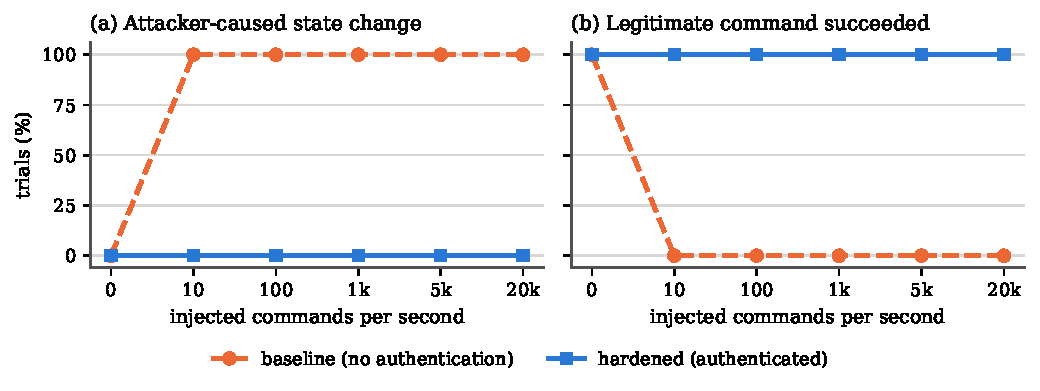
\includegraphics[width=\columnwidth]{fig_campaign.pdf}
\caption{Effect of command-injection rate. Left: fraction of trials in which the attacker
changed the system state. Right: fraction in which the legitimate command took effect. The
hardened build is flat across five orders of magnitude of attack intensity.}
\label{fig:campaign}
\end{figure}

\textbf{Fuzzing.} The command parser is the one input a network peer fully controls. We fuzz it
with the firmware built under AddressSanitizer and UndefinedBehaviorSanitizer, feeding random
bytes, malformed and overlong fields, non-decimal and overflowing counters, embedded NULs, and
bit-flip mutations of a near-miss signed message. After every input we check memory safety and
the invariant that no input lacking a valid tag changes state or advances the counter. Across
3{,}000{,}000 iterations the fuzzer found no memory error and no accepted input.

\section{The Open Step: Hardware Latency Invariance}\label{sec:hw}
The campaign establishes logical invariance; it cannot establish \emph{timing} invariance,
because the simulated clock does not model CPU or interrupt contention. That is precisely the
property in question on a single-chip SoC, and it can only be measured on silicon. We specify
the apparatus: an independent ESP32 times the interval from the PIR line to the siren line with
its own hardware timer (so the measuring clock is never the clock under load), across four
conditions---idle, heavy legitimate traffic, command-interface stress, and radio-layer stress
in an authorized isolated environment---and the same non-parametric test compares each loaded
condition against idle. A null result confirms that core pinning isolates the safety function on
this class of device, extending~\cite{fischer2020} to single-chip Wi-Fi SoCs; a positive result
would show it does \emph{not}, directly challenging standard practice. We report the protocol
rather than a number, and do not speculate on the outcome.

\section{Threats to Validity and Ethics}
Simulation shows logical, not physical, invariance (addressed by Section~\ref{sec:hw}).
Results are for one SoC family and one firmware; generalisation is a stated limitation. Latency
must be measured externally, not by the device under load. All adversarial radio work is
confined to an owned, isolated environment with permission; no third-party network is targeted,
and this paper deliberately omits any attack-generation procedure.

\section{Conclusion}
We cast a consumer intrusion alarm as a safety-critical system and asked whether the standard
single-chip mitigation---pin the safety task to a core---actually isolates it from attacks on
the device's own radio and command interface. We answer the logical half of that question with
exhaustive model checking and a 6{,}000-trial reproducible campaign, add the command
authentication, attack detection and fallback a deployable alarm needs, and specify the one
hardware measurement that settles the timing half. The artifact is public so the result can be
reproduced and the hardware step completed.

\begin{thebibliography}{9}
\small
\bibitem{fischer2020} F.\ Fischer \emph{et al.}, ``Analysis of Industrial Device Architectures
for Real-Time Operations under Denial of Service Attacks,'' arXiv:2007.08885, 2020.
\bibitem{carbajal2026} A.\ Carbajal and A.\ Jodeiri Akbarfam, ``A Software-Defined Testbed for
Quantifying Deauthentication Resilience in Modern Wi-Fi Networks,'' arXiv:2602.23513, 2026.
\bibitem{mqtttls2026} M.\ A.\ Azhar, M.\ Azwar, and O.\ Asroni, ``Performance and Security
Analysis of MQTT over TLS on ESP32-Based IoT Systems,'' \emph{J.\ Applied Informatics and
Computing}, 2026.
\bibitem{ondevice2026} V.\ Ieropoulos \emph{et al.}, ``Empowering IoT Security: On-Device
Intrusion Detection in Resource Constrained Devices,'' arXiv:2605.13159, 2026.
\bibitem{mcreview2026} A.\ Burns and R.\ I.\ Davis, ``Mixed Criticality Systems: A Review,''
14th edn., Dept.\ of Computer Science, University of York, Feb.\ 2026.
\bibitem{timingiso2025} L.\ Meszl\'enyi, J.\ Kahle, D.\ P\"ullen, S.\ Kowalewski,
S.\ Katzenbeisser, and A.\ Kampmann, ``Towards Timing Isolation for Mixed-Criticality
Communication in Software-Defined Vehicles,'' arXiv:2508.13652, 2025.
\bibitem{mcti2024} D.\ Hoornaert, G.\ Ghaemi, A.\ Bastoni, R.\ Mancuso, M.\ Caccamo, and
G.\ Corradi, ``Mcti: mixed-criticality task-based isolation,'' \emph{Real-Time Systems},
vol.\ 60, no.\ 2, pp.\ 328--365, 2024.
\bibitem{deauther2026} S.\ Kremser and K.\ Graffi, ``Evaluating the ESP32-S3 for Wi-Fi
Penetration Testing Through the Development of Deauther32 and HackHeld32,'' \emph{Sensors},
vol.\ 26, no.\ 11, art.\ 3287, 2026.
\bibitem{espwn2023} R.\ Cayre, D.\ Cauquil, and A.\ Francillon, ``ESPwn32: Hacking with ESP32
System-on-Chips,'' in \emph{Proc.\ 17th IEEE Workshop on Offensive Technologies (WOOT)}, 2023.
\bibitem{krichen2023} M.\ Krichen, ``A Survey on Formal Verification and Validation Techniques
for Internet of Things,'' \emph{Applied Sciences}, vol.\ 13, no.\ 14, art.\ 8122, 2023.
\bibitem{lamport2002} L.\ Lamport, \emph{Specifying Systems: The TLA+ Language and Tools for
Hardware and Software Engineers}. Addison-Wesley, 2002.
\bibitem{fuzzsurvey2022} J.\ Yun \emph{et al.}, ``Fuzzing of Embedded Systems: A Survey,''
\emph{ACM Computing Surveys}, 2022.
\bibitem{pemu2025} M.\ Bley, T.\ Scharnowski, S.\ W\"orner, M.\ Schloegel, and T.\ Holz,
``Protocol-Aware Firmware Rehosting for Effective Fuzzing of Embedded Network Stacks,'' ACM,
2025, doi:10.1145/3719027.3765125.
\bibitem{sysfuss2026} D.\ Tharindu, A.\ Jayasena, and P.\ Mishra, ``SysFuSS: System-Level
Firmware Fuzzing with Selective Symbolic Execution,'' arXiv:2602.02243, 2026.
\end{thebibliography}

\end{document}
